\chapter{二维硼化钛的超导电性}

% 硼元素因为具有独特的多中心键,其化合物在低维时能够展现出丰富的结构多样性。
% 现在已经被实验发现的,就包括许多的零维硼团簇和二维硼平面。
% 在稳定的硼团簇中,\ce{B12}\cite{kiran2009origin}是最为稳定的结构之一,
% 它可以被看作是平面三角网格的零维碎片。当原子数持续增加,硼平面团簇的结构中会出现空位,
% 这样六边形空位的出现使得团簇更稳定。在\ce{B30}和\ce{B36}\cite{pham2014boron}中都存在这样的空位,
% 而这样具有空位的结构是该原子数的硼团簇中最为稳定的。

% 过渡到二维硼平面,为了平面结构在能量上更加稳定,同样需要在结构中出现如团簇平面中的六角形空位。
% 在已经被理论计算预言的稳定的硼单层平面中,$\alpha$-硼平面\cite{yang2008ab}的单胞中就有硼六角空位。
% 根据该结构规律,我们课题组先前的工作中\cite{xu2017practical},给出了一系列具有相似结构特征的稳定硼平面结构,
% 并总结了硼平面结构稳定的结构规律与化学原因。此外,其他课题组还发现了许多硼平面结构的新奇物理化学性质,
% 如超导电性\cite{penev2016can,zhao2016superconductivity},拓扑性质\cite{feng2017dirac},
% 二维硼半导体\cite{xu2017two}等。

通过在硼平面或硼团簇中嵌入金属元素,尤其是过渡金属元素,硼元素化合物的结构多样性会变得更加的丰富,也因此能够表现出更为丰富的性质。
比如,准单层的\ce{TiB2}结构的能带中可以观察到狄拉克锥\cite{zhang2014prediction},其费米能级处的电子迁移率能够和石墨烯媲美。
二维的\ce{MoB4}\cite{xie2014first}则在费米能级处有双狄拉克锥,同样有极好的电子迁移率。
实验上,已经发现了许多过渡金属与硼构成的稳定多配位平面团簇结构\ce{TM}@\ce{B_n}。
我们认为,这些过渡金属硼平面团簇结构,可以看作是过渡金属硼平面的结构碎片,从而充当构成稳定过渡金属硼平面的构筑单元。
相似的已经报导的过渡金属硼化物还包括,
理论计算预测第四周期过渡金属硼平面中,\ce{FeB6}\cite{li2016global}为半导体,\ce{CrB4}\cite{li2019room}为单层铁磁材料并有高达\SI{401}{\kelvin}的居里温度。

而过渡金属因其未配对的$d$轨道电子,还会展现出丰富的磁学和电学性质。
超导电性作为一种有重要实用与理论研究价值的性质,该性质是否能够出现在金属-硼构成的二维材料中,是一个有趣且有研究价值的问题。
已经被理论预测报导的金属-硼二维超导材料有\ce{Mo2B2}\cite{yan2019prediction},\ce{Li-B}单层\cite{wu2016lithium}。
本章主要介绍过渡金属钛与硼元素构成稳定的过渡金属单层硼平面,其中\ce{TiB7}最稳定的单层构型,表现出超导电性。

为探究潜在的超导电性,在下面的章节中首先介绍超导电性的计算方法,
再详细分析\ce{TiB7},\ce{TiB9}单层和\ce{TiB7}双层的电声耦合和超导电性。

\section{电声耦合和超导电性的计算}
从Fr{\"o}hlich哈密顿量\cite{frohlich1954theory}出发我们可以得到电子之间的相互作用满足以下关系:
\begin{equation}
  V_{\mathrm{eff}}(\bm{k},-\bm{k},\bm{q}) = |g_{\bm{k},\bm{q}}|^2
  \frac{\omega_{\bm{q}}}{(\epsilon_{\bm{k}}-\epsilon_{\bm{k}+\bm{q}})^2-\omega^2_{\bm{q}}} ,
\end{equation}
其中$g_{\bm{k},\bm{q}}$为耦合函数描述了体系中电子和声子的耦合,可以通过下面关系得到,所需要的参数都可以从体系电子结构和声子谱的第一性原理计算中得到:
\begin{equation}\label{eq:coupling_coeff}
  g^{\bm{q}\lambda}_{\bm{k}+\bm{q}\nu',\bm{k}\nu} =
  \sum_{\kappa\alpha} A^{\bm{q}j}_{\kappa\alpha}
  \langle {\bm{k}+\bm{q}\nu'} | {\delta^{\bm{q}}_{\kappa\alpha}v_{\mathrm{eff}}} | {\bm{k}\nu} \rangle ,
\end{equation}

超导电性是电子系统体现的宏观现象。它源于由于低于临界温度时,体系所处的费米液体态不稳定而向更稳定的新的电子和电子成对(库伯对)的基态过渡。BCS理论\cite{bardeen1957theory}展示的是,当体系中两个电子存在吸引相互作用时,该电子电子成对的状态是稳定的。而这个电子电子成对的吸引力就是由电声耦合提供的。电声耦合(EPC)是已知的大多数的超导现象的来源,这类超导通常被称为常规超导体以区别其他材料中存在的尚未有完全清楚的理论机制的成对相互作用而导致的超导。

BCS理论,假设了电声耦合是弱耦合。后续在BCS基础上应用多体系统处理的方法\cite{scalapino1969electron}发展而来的Elishberg理论\cite{eliashberg1960interactions}将BCS理论中的弱耦合拓展到了强耦合,从而可以定量的预测许多超导态的性质。
超导态的一个重要性质是其准粒子的谱上有一个带隙,带隙的大小是超导电性的一个重要的序参量。
Elishberg理论的一个重要的结果是其描述超导能带的方程的计算中不需要用到体系的超导态而只需要特定体系的正常电子态的信息。包括体系的电子结构和声子调制的电子成对能,这些信息通过第一性原理和上面的电声耦合的计算就能得到。

在本论文中我将省略Eliashberg理论的导出而仅仅列出其在超导电性计算中所用到的结果,和有效电子电子相互作用的计算过程。声子调制的电子电子相互作用是两个电子之间通过交换一个声子的物理过程,可以由下列的Eliashberg函数表示:
\begin{equation}\label{eq:elishaberg_aniso}
  \alpha^2 F_{\bm{k}\nu,\bm{k}'\nu'}(\omega) =
  N(\epsilon_F) \frac{1}{N_{\bm{q}}} \sum_{\bm{q}j}
  |g^{\bm{q}j}_{\bm{k}'\nu',\bm{k}\nu}|^2 \delta(\omega-\omega_{\bm{q}j}) ,
\end{equation}
其中的$N(\epsilon_F)$是费米能级处单个电子的电子态密度。在固定频率$\omega$对所有该过程涉及的声子模式求和。耦合的相互作用就是前面提到的包含屏蔽效应的电声相互作用耦合函数(矩阵元表示)即式(\ref{eq:coupling_coeff})。该式右边只涉及非超导态的性质。又由于动量守恒,在该过程中$\bm{q}=\bm{k}-\bm{k}'$。且该电子成对相互作用形成的过程中,有效的电子态集中在能量为,$|\epsilon_{\bm{k}\nu}-\epsilon_F|<\omega_{\mathrm{phonon}}$处,因此在式(\ref{eq:elishaberg_aniso})中可以仅仅考虑费米面处的电子\cite{allen1983theory}。

大多数超导体都表现出各向同性的超导带隙,原因是真实材料中都存在缺陷,而缺陷的存在会抵消电子相互作用的动量依赖。根据这两个假设,在大多数情况下可以近考虑费米面附近的电子态,且使用各项同性的Elishaberg函数:
\begin{equation}\label{eq:elishaberg_iso}
  \alpha^2 F(\omega) = \frac{1}{N(\epsilon_F)}\frac{1}{N_{\bm{q}}}
  \sum_{\substack{\bm{q}j \\ \bm{k}\nu\nu'}} |g^{\bm{q}j}_{\bm{k}+\bm{q}\nu',\bm{k}\nu}|^2
  \delta(\omega-\omega_{\bm{q}j})
  \delta(\epsilon_{\bm{k}\nu}-\epsilon_{F})
  \delta(\epsilon_{\bm{k}+\bm{q}\nu'}-\epsilon_F) ,
\end{equation}
在Elishaberg理论中重要的宏观物理量如超导转变温度都是对全频率的积分形式。各项同性的耦合常数可以表示为:
\begin{equation}\label{eq:lambda_coupling}
  \lambda = 2 \int d\omega \frac{\alpha^2 F(\omega)}{\omega} ,
\end{equation}
该量是一个无量纲的量,描述了体系电声耦合的平均强度。由积分内的$1/\omega$可以看出在电子成对形成过程中低频的声子的贡献要比高频的声子的贡献更大。

利用$T\rightarrow 0$时的声子线宽$\gamma_{\bm{q}j}$的表达式,可以将Elishaberg函数写为下列形式:
\begin{equation}\label{eq:elishaberg_calc}
  \alpha^2 F(\omega) = \frac{1}{2\pi N(\epsilon_F)}\frac{1}{N_{\bm{q}}}
  \sum_{\bm{q}j} \frac{\gamma_{\bm{q}j}}{\omega_{\bm{q}j}}
  \delta(\omega-\omega_{\bm{q}j}) ,
\end{equation}
代入式(\ref{eq:lambda_coupling})得耦合常数:
\begin{equation}
  \lambda = \frac{1}{\pi N(\epsilon_F)}\frac{1}{N_q}
  \sum_{\bm{q}j}\frac{\gamma_{\bm{q}j}}{\omega^2_{\bm{q}j}} ,
\end{equation}
从这个形式可以看出,Elishaberg函数是对所有的声子分支进行积分中再对声子的动量求平均。

在用DFPT方法计算Elishaberg函数的实际操作中,首先对声子线宽进行计算再对其在全部声子频率求和得到。式(\ref{eq:elishaberg_calc})中的$\delta$函数在实际数值计算时通常使用平滑的高斯函数来代替,为了达到该近似的收敛往往需要很密的$k$点。而很密的$k$的计算可以使用Wannier函数来得到,该方法被称为电声耦合Wannier函数方法\cite{ponce2016epw}。

Fr{\"o}hlich哈密顿量的电子部分没有考虑电子电子本来的库伦相互作用(哈密顿量中电子部分由单粒子算符表示)。电子电子间的库伦相互作用在结果中主要影响的是式(\ref{eq:elishaberg_iso})中准粒子的本征值$\epsilon$以及相应的声子的本征值$\omega$。实际物理过程包含有电子间的库伦相互作用,因此我们不能在声子调制的超导电性的计算中忽略这个相互作用,因为这个相互作用是排斥的因此会大大抑制前面导出的成对相互作用(吸引)。与电声耦合参数类似,可以引入所谓库伦参数来描述这个相互作用,即费米面处的平均有效库伦屏蔽。因为电子比晶格振动在时间尺度上快的多,因此能量上也比声子大的多,我们再定义Morel-Anderson库伦赝势\cite{morel1962calculation}来描述不同声子频率上限下的库伦参数:
\begin{equation}
  \mu = N(0)\langle\langle {V_C(k,k')} \rangle\rangle_{FS}
\end{equation}
\begin{equation}
  \mu^*(\omega_c) = \frac{\mu}{1+\mu \ln(\varepsilon_0/\omega_c)} ,
\end{equation}
$\varepsilon_0$为电子系统的特征能量尺度,同时引入了一个比声子能大得多的截止$\omega_c$。在本论文的工作中我们使用了经验值来设置该参数$\mu^*$。实际上还可以通过更精确的超导第一性原理来计算得到这个参数\cite{kohn1989orbital}。

超导转变温度$T_c$仅仅依赖于与材料相关的物理量$\alpha^2 F(\omega)$和$\mu^*$的值。
Allen和Dynes\cite{allen1975transition}对各向同性带隙方程进行了深入的数值分析,
他们使用了一套$\alpha^2 F(\omega)$的标准谱,并在很大的参数范围内改变$\lambda$和$\mu^∗$。
他们的研究揭示了这样一个重要结论,即他们发现在一个较小的参数空间(即$\lambda<2$和$\mu^∗<0.15$)中,$T_c$可以很好地近似于最初由McMillan\cite{mcmillan1968transition}提出的$T_c$公式,不同的是需要加入一个修正的前因子:
\begin{equation}\label{eq:tc}
  T_c = \frac{\omega_{\mathrm{log}}}{1.2}
  \exp{\left[ {-\frac{1.04(1+\lambda)}{\lambda-\mu^*(1+0.62\lambda)}} \right]} ,
\end{equation}
前置因子包含了声子谱的平均频率(以对数方式定义的平均值),并与耦合强度加权平均,
\begin{equation}
  \omega_\mathrm{log} = \exp \left[ {\int d\omega \log(\omega)W(\omega)} \right],
\end{equation}
其中的权重$W$定义为:
\begin{equation}
  W(\omega) = \frac{2}{\omega} \frac{\alpha^2 F(\omega)}{\omega} ,
\end{equation}
该Tc公式是对弱耦合极限下BCS公式$T_c = 1.13 \omega_D \exp(−1/\lambda)$的改进。

\section{单层\ce{TiB7}的超导电性}

\begin{figure}
  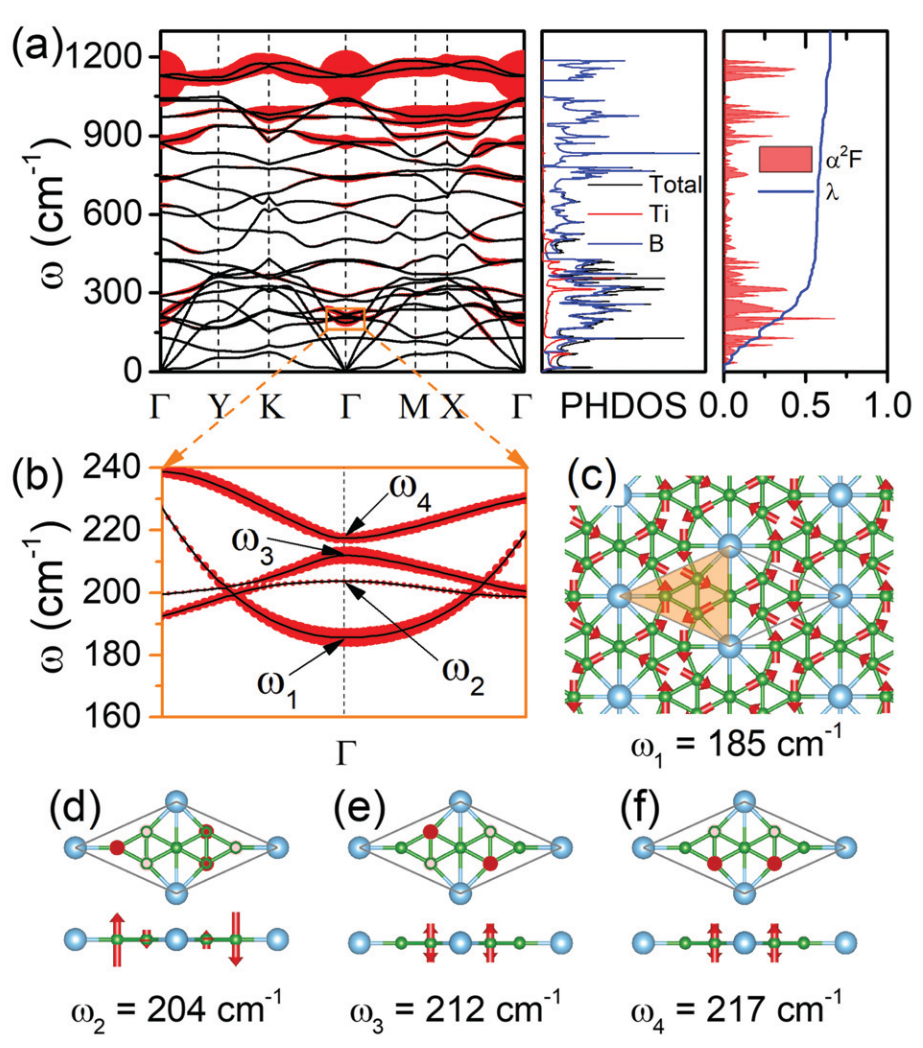
\includegraphics[width=0.96\textwidth]{figs/ch5_tib7_sc_all.png}
  \centering
  \caption{(a)红色包围的区域中声子色散与声子线宽$\gamma_{qj}$、
  声子态密度以及单层\ce{TiB7}的Eliashberg函数$\alpha^2 F(\omega)$和$\lambda(\omega)$。
  (b)$\Gamma$点附近频率从\SI{160}{\per\cm}到\SI{240}{\per\cm}处的声子谱放大图
  (c)$\omega_1$面内剪切模,
  (d-f)垂直于面平面的呼吸模。
  红色箭头及其长度代表了相应振动模式的方向和振幅。}
  \label{fig:ch5_tib7_sc_all}
\end{figure}

图\ref{fig:ch5_tib7_sc_all}展示了\ce{TiB7}单层的声子谱
及各个振动模式不同频率的声子线宽$\gamma_{\bm{q}j}$,
Eliashhberg函数$\alpha^2 F(\omega)$和$\lambda(\omega)$ 。
首先可以确定的是,结构可以在单层状态稳定存在,
因从图\ref{fig:ch5_tib7_sc_all}(a)的\ce{TiB7}声子谱中没有虚频。

从图中可以看出,主要是低频($<$\SI{400}{\per\cm})的振动模式贡献了电声耦合。
从Eliashberg函数$\alpha^2 F(\omega)$可看出,在频率为约\SI{200}{\per\cm}处有数个尖峰,
其主要是由该频率位于$\Gamma$点周围的声子贡献的,此处在$\Gamma$点的声子线宽较大。
虽然在高频处,当频率大于\SI{900}{\per\cm}时,明显可见该位置的声子线宽很大。
特别是在$\Gamma$点附近,描述声子线宽的红色区域覆盖了很宽的频率范围。
从Eliashberg函数随声子能量的变化也能看出,
在声子频率大于\SI{900}{\per\cm}时,有数个尖峰,且尖峰的面积也较大,
说明该高频区域的声子对Eliashberg函数有很大的贡献。
然而,真正对超导温度起到影响作用的直接宏观物理量是电声耦合常数,
其形式为对全频率的积分,且该物理量对声子频率平均,
即越大的频率对耦合常数$\lambda$贡献更小。
直观上这也符合声子对电子成对所造成的影响,我们可以认为声子频率和晶格
中原子的振动频率直接关联,若某个振动模式频率很大,原子振动很快,
则原子来不及在其振动的平衡位置形成有效的电荷中心和电子发生相互作用。
取极端情况来描述这个现象,即当声子频率无穷大时,可近似认为
原子不振动而只是其原子半径变大(变为振动半径),这时模型等价于
完美晶格,电子和声子无耦合。
从图\ref{fig:ch5_tib7_sc_all}(a)中耦合常数$\lambda$的变化可知,
高频处的声子对耦合常数的贡献很小。

我们将$\Gamma$点附近频率从\SI{160}{\per\cm}到\SI{240}{\per\cm}处的声子谱放大在
图\ref{fig:ch5_tib7_sc_all}(b)中展示,
此处有四种振动模式$\omega_1$、$\omega_2$、$\omega_3$和$\omega_4$,
分别代表了如图\ref{fig:ch5_tib7_sc_all}(c-f)所示的四种振动。
其中,$\omega_1$为面内的剪切模,如图\ref{fig:ch5_tib7_sc_all}(c),
它的振动模式的对称性为$C_3$。图\ref{fig:ch5_tib7_sc_all}(d-f)为其余三个垂直于面平面的振动模式,
通常在文献中,将这种垂直于面的振动模式称为呼吸模。
在四种模式中,剪切模$\omega_1$和呼吸模$\omega_3$、$\omega_4$的声子线宽较大。
$\omega_2$处的声子线宽较小,但由于其该带很平,在态密度中这一频率处贡献很大。
综上两个因素导致了在\SI{200}{\per\cm}附近Eliashberg函数的绝对值较大,贡献了很大的电声耦合。
根据McMillan-Allen-Dynes参数化Eliashberg方程,式\ref{eq:tc},我们可以估计超导临界温度$T_c$。

根据之前关于硼材料研究的文献\cite{penev2016can,zhao2016superconductivity,zhao2018multigap,liao2017phonon,yan2020superconductivity},
上面经验公式中的库伦排斥势$\mu^*$我们选取了$\mu^*=0.1$来计算超导转变温度。
图\ref{fig:ch5_tib7_coupling}中展示了电声耦合系数$\lambda_{\bm{q}j}$在倒空间中的变化情况,
我们可以看到,在$\Gamma$点附近是一个以$\Gamma$点为中心的哑铃形状的分布,
其最大的$\lambda_{\bm{q}j}$值大于\num{1.0}。
全部倒空间中的电声耦合系数除了$Y$对称点处均大于\num{0.6}。
因而总的电声耦合常数$\lambda$为\num{0.65}。
将$\lambda$代入以上公式中我们得到单层\ce{TiB7}平面的超导转变温度为\SI{8.3}{\kelvin}。
该超导温度高于报导的锂沉积石墨烯的超导转变温度,即理论计算的超导温度为\SI{8.1}{\kelvin}\cite{profeta2012phonon},
实验测量得到的超导转变温度为\SI{5.9}{\kelvin}\cite{ludbrook2015evidence}。
在钛硼化合物中,原子质量较小的硼元素是常规BCS超导电声耦合的主要原因。
同样的所有的单层金属硼平面均显示出超导电性,而超导转变温度和硼平面的空位浓度之间存在先减少后增加的关系。
当空位浓度为\num{1/9}时,最稳定的$\alpha$-硼平面的超导转变温度为\SI{3.7}{\kelvin}。
当空位浓度增加到\num{1/8}时超导转变温度提高到\SI{5.8}{\kelvin}。
我们可以看到,通过引入钛原子增加里材料的电声耦合并提高了超导转变温度$T_c$。
钛单质块体中测量得到的超导转变温度最大为\SI{0.38}{\kelvin}\cite{matthias1963superconductivity},
因此在\ce{TiB7}中超导主要是由硼元素所贡献的。

\begin{figure}
  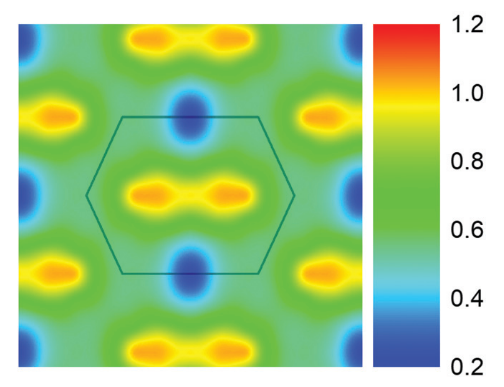
\includegraphics[width=0.72\textwidth]{figs/ch5_tib7_coupling.png}
  \centering
  \caption{\ce{TiB7}电声耦合系数$\lambda_{\bm{q}j}$在倒空间中的变化情况}
  \label{fig:ch5_tib7_coupling}
\end{figure}

二维BCS型超导体\ce{AlB6}中报导了通过拉伸材料可以提高,\SI{12}{\percent}的拉伸应变可以将超导温度提高到30K。
这通常是由于,对平面结构的拉伸使得原子间的距离变得更远,
原子间的相互作用变弱,对于高频处声子原子间互相作用变小
会使得原子的振动频率降低,但同时声子线宽也通常会变小。
但一般来说,高频处有较大的声子线宽,
如果拉伸能够使得高频处声子的频率快速较低而对
耦合常数带来快速的提升,则拉伸应变会大大提高超导温度。

我们同样对\ce{TiB7}平面作了相似的拉伸应变,从图\ref{fig:ch5_tib7_strain}中可以看到,
如预期,拉伸应变使得频率较高、线宽较大的声子的频率降低。
频率最高的两支声子的频率从无拉伸应变时的范围\SI{1000}{\per\cm}至\SI{1200}{\per\cm}
下降至\SI{5}{\percent}拉伸时的频率范围变为\SI{800}{\per\cm}至\SI{1000}{\per\cm}之间。
声子频率的下降说明声子能量的下降,与之同步变化的是,
可以看到,随着拉伸应力增大,声子线宽变即声子谱中高频声子所包围的红色区域面积在变小。
但是即便有较大线宽的声子模式的频率下降,但其对耦合常数的贡献依然很弱,
如前所述,拉伸应变反而使得超导临界温度降低。
我们分析,\ce{TiB7}单层构型的电声耦合主要来自低频处的四个声子模式。
四个声子模式中,仅有面内的$\omega_1$振动模式(图\ref{fig:ch5_tib7_sc_all}(c))
随着拉伸频率下降(但声子线宽也变小),其余三个呼吸模的频率均随着
拉伸应力的增大而增大,综合效果是整体的耦合常数减小,
超导临界温度降低。

\begin{figure}
  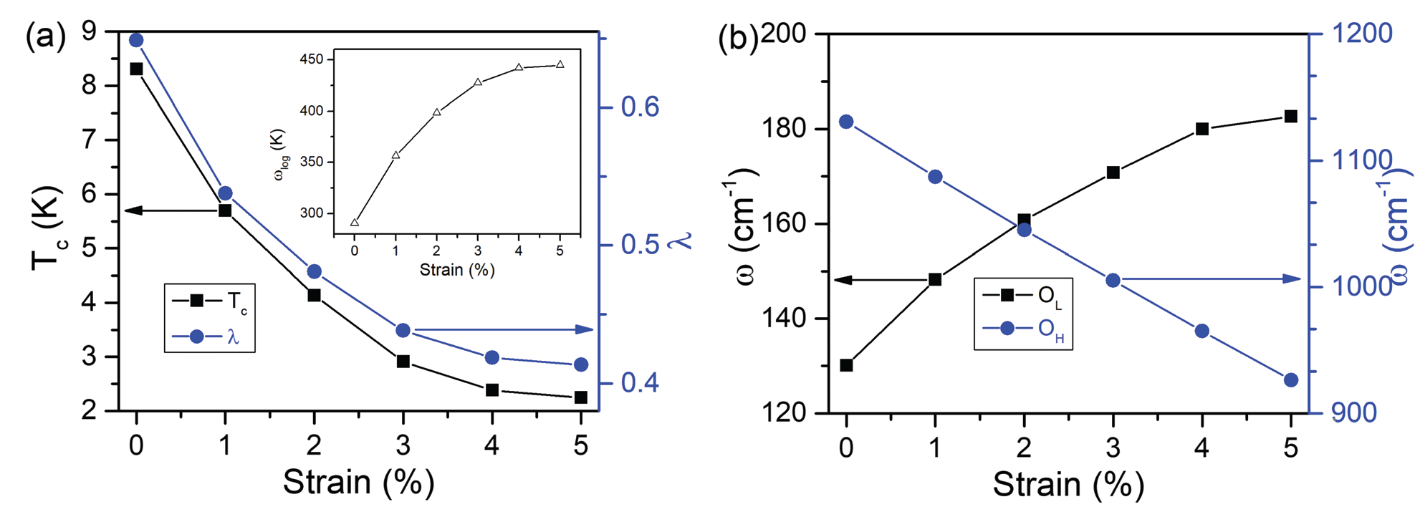
\includegraphics[width=0.96\textwidth]{figs/ch5_tib7_strain.png}
  \centering
  \caption{(a)\ce{TiB7}单层的$T_c$和电声耦合常数$\lambda$随等双轴拉伸应变的变化。
  内插图为对数平均声子频率($\omega_{\mathrm{log}}$)的变化。
  (b)在$\Gamma$处的声子光学支的最低($O_L$)和最高($O_H$)频率随应变变化的函数。}
  \label{fig:ch5_tib7_strain}
\end{figure}

结合声子态密度图,低频率的声子频率范围恰好与\ce{Ti}原子的声子态密度贡献重合,
说明虽然原子质量较小的硼原子是电声耦合效应的直接来源,
但钛原子支撑力结构,并使得低频处的这四个对超导电性有正面贡献的
声子模式得以出现。

综上,拉伸并没有提高超导温度,在施加\SI{5}{\percent}的拉伸应变后材料的超导转变温度降低到了约2K。
尽管随着应力的增加$\omega_\mathrm{log}$持续增加,但是总的电声耦合常数和超导转变温度均减小。
其中,$\Gamma$点处低频的声子频率随应力增加而增加,高频的声子频率随应力的增加而减少。
图\ref{fig:ch5_tib7_strain}中展示了高频声子和低频声子频率随拉伸应变的变化关系。
我们还在图\ref{fig:ch5_details_strains}中展示了声子谱以及Eliashberg函数随应力变化的详细关系。

\begin{figure}
  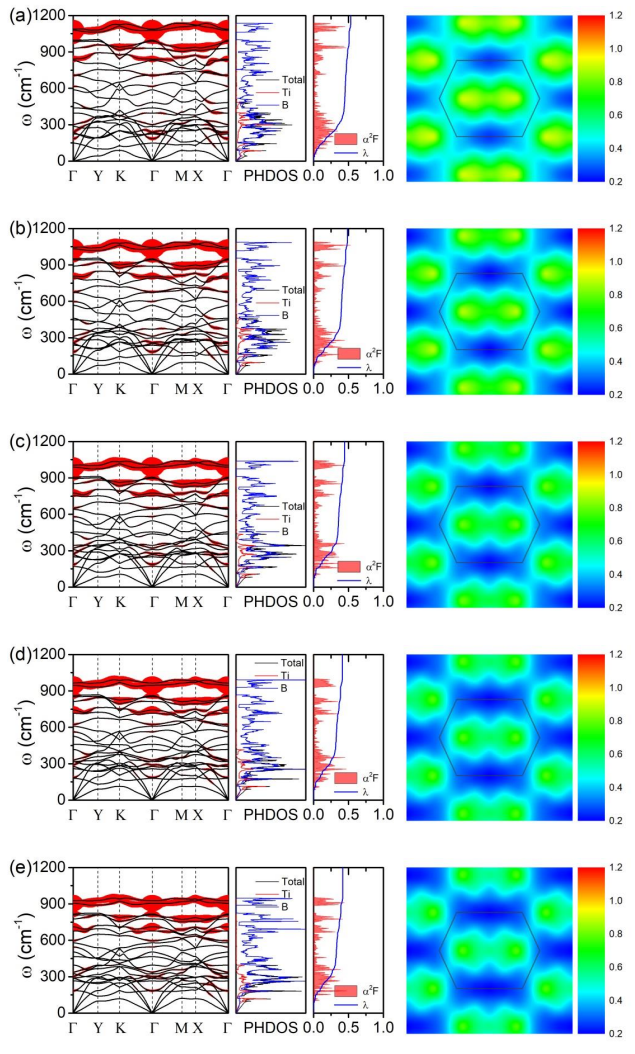
\includegraphics[width=0.88\textwidth]{figs/ch5_details_strains.png}
  \centering
  \caption{在拉伸应变为(a)\SI{1}{\percent},(b)\SI{2}{\percent},(c)\SI{3}{\percent},(d)\SI{4}{\percent},(e)\SI{5}{\percent},\ce{TiB7}单层薄膜的声子色散以及声子线宽$\gamma_{qj}$、声子态密度、
  Eliashberg函数$\alpha^2 F(\omega)$和$\lambda(\omega)$和耦合常数强度在倒空间的分布。}
  \label{fig:ch5_details_strains}
\end{figure}

若拉伸应变会减小超导转变温度,则相反的压缩应变应该增加超导转变温度,
如\ce{B5}硼平面\cite{cheng2017suppressed},二维\ce{TiS2}\cite{liao2020doping},
甚至并非属于BCS超导的\ce{FeS}层状结构\cite{nie2009suppression}。
然而,对于\ce{TiB7}单层压缩应变在达到\SI{1}{\percent}后结构声子谱中就出现
了如图\ref{fig:ch5_tib7_tib9_pd}(b)中的严重的虚频,我们认为该强度的应变就会使结构出现相变。

作为对比,我们还计算了\ce{TiB9}单层的超导相关性质。如图\ref{fig:ch5_tib9_phonon},
该结构声子谱中同样不存在虚频说明其能够以二维的形式稳定存在。
电声耦合的计算结果如图\ref{fig:ch5_tib9_phonon}所示,
其各向同性平均电声耦合系数$\lambda$为0.40。
在$\Gamma$点附近其电声耦合系数最大为$\lambda_{\bm{q}j}$约为0.7。
由此可以估计其超导转变温度为\SI{1.2}{\kelvin}。如前面描述的,\ce{TiB7}单层是完全平面的结构,
而\ce{TiB9}不同其垂直方向有原子的起伏。
为了研究垂直方向的起伏对超导电性的影响,我们希望能够构造了完全平整的\ce{TiB9}构型作为对比,
研究其声子部分振动模式信息的变化作为参照,以确定是否完全平整的平面能够提高电声耦合从而提高超导电性。
优化后的\ce{TiB9}平面构型的晶格参数增加了\SI{1.2}{\percent},且总能上升了\SI{0.19}{\eV}。
然而,计算结果显示该构型有明显的虚频如图\ref{fig:ch5_tib7_tib9_pd}(a)所示,因此无法进一步研究电声耦合性质以作为对比。

\begin{figure}[htb]
  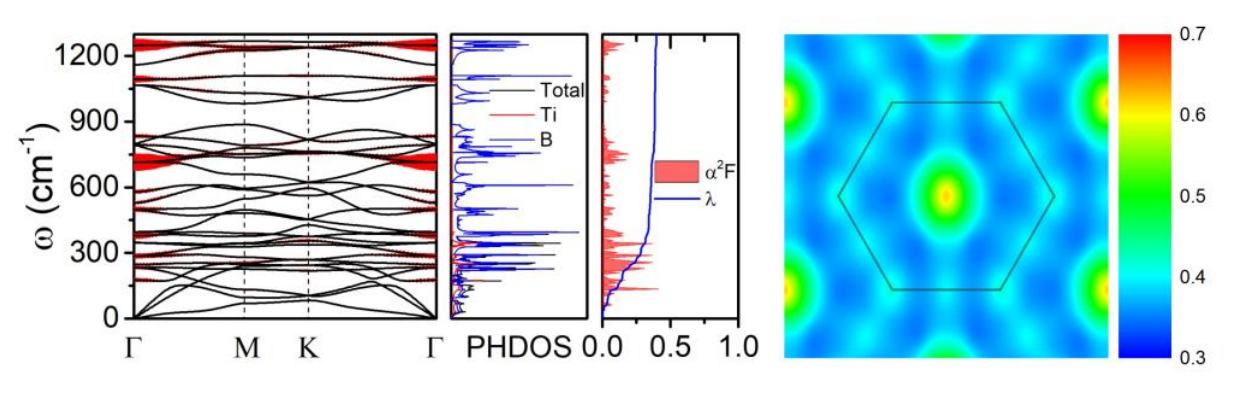
\includegraphics[width=0.96\textwidth]{figs/ch5_tib9_phonon.png}
  \centering
  \caption{\ce{TiB9}单层薄膜的声子色散以声子线宽$\gamma_{qj}$、声子态密度、Eliashberg函数$\alpha^2 F(\omega)$和$\lambda(\omega)$和耦合常数强度在倒空间的分布。}
  \label{fig:ch5_tib9_phonon}
\end{figure}

\begin{figure}
  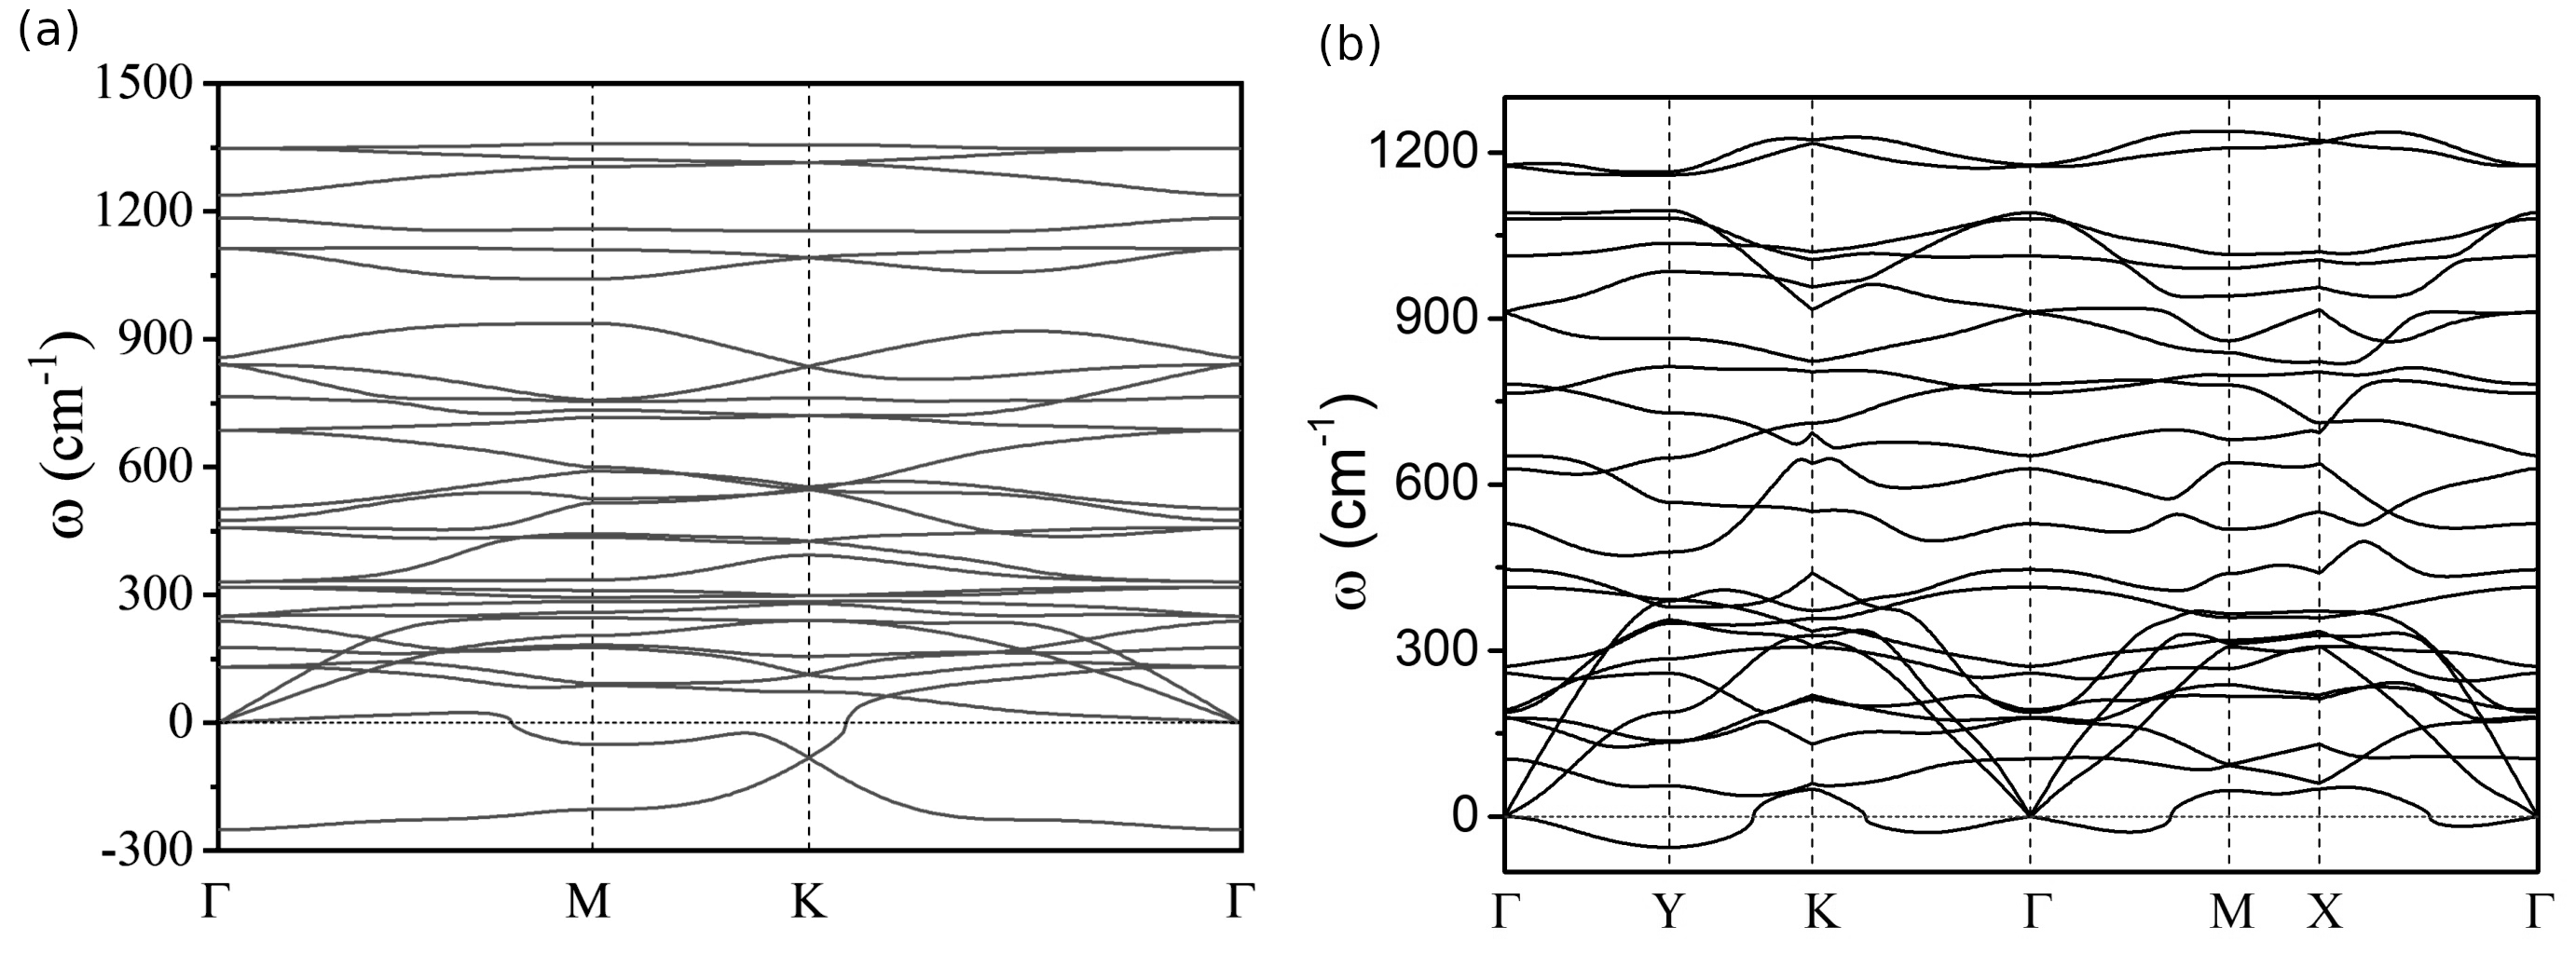
\includegraphics[width=0.96\textwidth]{figs/ch5_tib7_tib9_pd.png}
  \centering
  \caption{(a)全平的\ce{TiB9}的声子谱。(b)\ce{TiB7}单层压缩应变达到\SI{1}{\percent}后结构声子谱}
  \label{fig:ch5_tib7_tib9_pd}
\end{figure}

我们分析了\ce{TiB7}和\ce{TiB9}两个单层平面能带,
态密度和投影态密度等电子结构性质如图\ref{fig:ch5_bands}。
\ce{TiB7}和\ce{TiB9}均为金属,费米能级穿过其能带。
\ce{TiB7}单层费米能级附近的态主要是由钛的$d$轨道和硼的$p$轨道构成的,
而在\ce{TiB9}中,费米能级附近的波函数主要来自于钛的$d$轨道。
与\ce{TiB4}单层相比,$d$轨道能级在单层中构成了一个接近水平的能带,
这个轨道大大增加了费米能级附近的态密度,因此可能使其成为潜在的超导材料。

\begin{figure}[htb]
    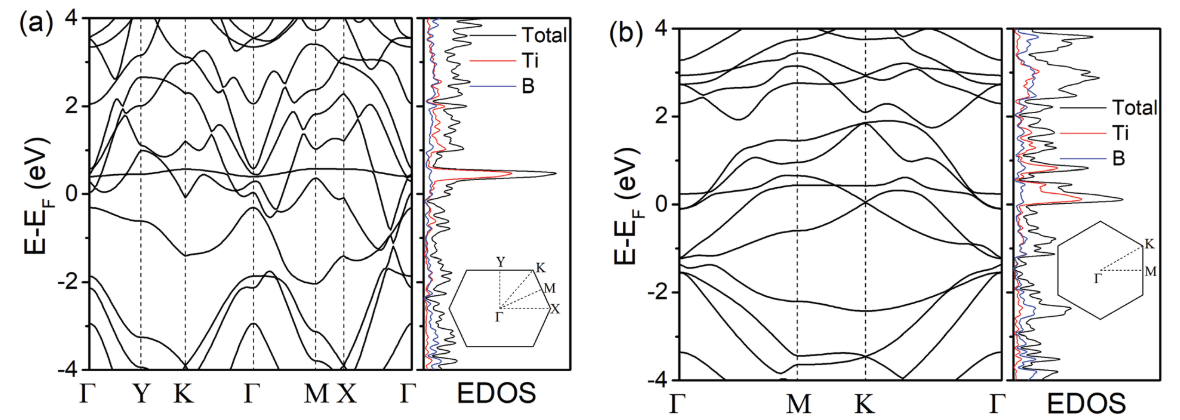
\includegraphics[width=0.96\textwidth]{figs/ch5_bands.png}
    \centering
    \caption{\ce{TiB7}和\ce{TiB9}的能带和态密度。}
    \label{fig:ch5_bands}
\end{figure}

\section{双层\ce{TiB7}的超导电性}
我们考虑通过将\ce{TiB7}堆积为双层构型是否能够提高其超导电性。
如图\ref{fig:stack-kinds}所示,可以有三种堆叠方式,
其中,AA型堆叠的层间结合能很弱,我们认为堆叠不会对其超导性质产生影响。
AB型堆叠的层间结合能最强,因此我们选择这个结构来进一步研究其超导电性。

\begin{figure}[H]
  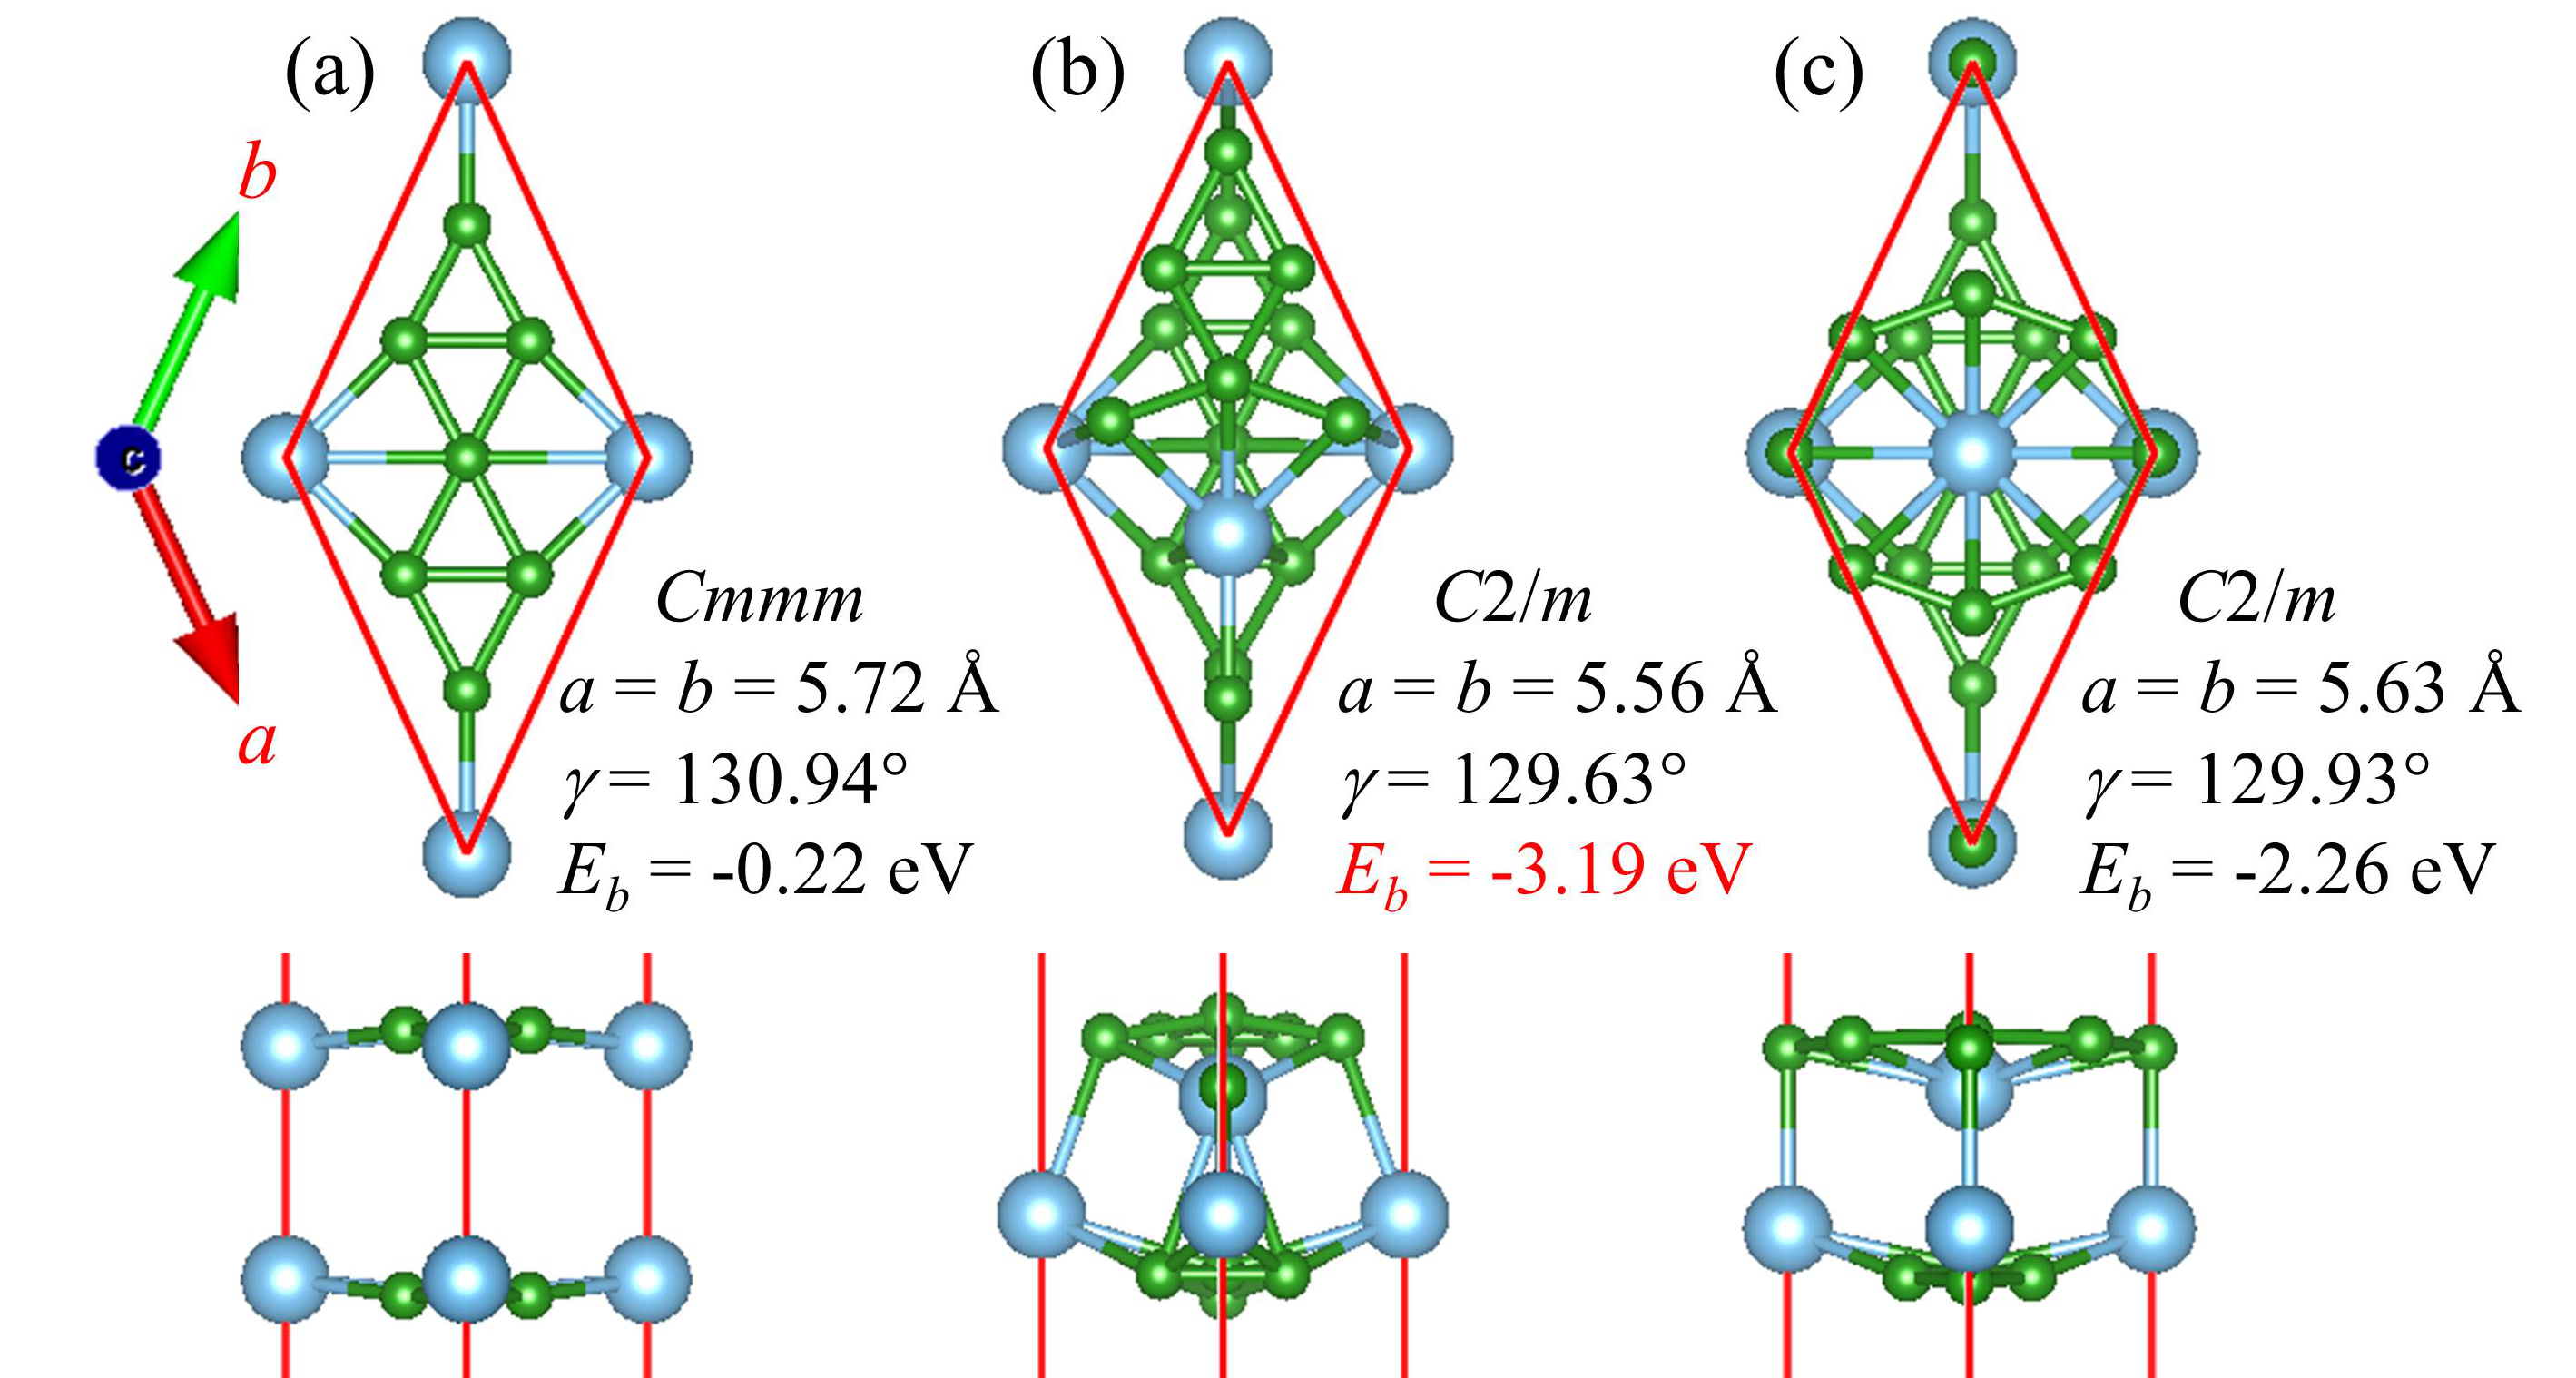
\includegraphics[width=0.96\textwidth]{figs/stack-kinds.png}
  \centering
  \caption{双层\ce{TiB7}原子结构的顶视图和侧视图,
  (a)AA堆叠,
  (b)AB堆叠(B层:\ce{Ti}原子在A层\ce{Ti}原子构成的三角形中心)和
  (c)AC堆叠(C层:\ce{Ti}原子在A层\ce{Ti}原子构成的菱形中心)。}
  \label{fig:stack-kinds}
\end{figure}

如下图\ref{fig:ch5_stack_tib7},展示了\ce{TiB7}单层堆叠后形成的双层的声子谱及声子线宽$\gamma_{\bm{q}j}$,
Eliashhberg函数$\alpha^2 F(\omega)$和$\lambda(\omega)$。
可以确定的是,从图\ref{fig:ch5_stack_tib7}的AB形式堆叠的\ce{TiB7}双层的声子谱可以看出,
声子谱中没有虚频说明结构可以在叠层状态稳定存在。
但相比于单层堆叠的\ce{TiB7}构型,双层的\ce{TiB7}费米能级处的电子密度$N(\epsilon_F)$下降了
近\SI{25}{\percent},
因此导致电声耦合系数$\lambda$下降了约\SI{22}{\percent},
超导转变温度下降了\SI{34}{\percent}。

从图中可以看出,在该双层构型中,同样是是低频($<$\SI{400}{\per\cm})的振动模式贡献了主要的电声耦合。
与单层\ce{TiB7}超导电性计算时相同,经验公式中的库伦排斥势$\mu^*$我们依然选取使用了$\mu^*=0.1$来计算超导转变温度。
根据McMillan-Allen-Dynes方程,我们可以估计超导临界温度$T_c$为\SI{5.5}{\kelvin}。
与单层\ce{TiB7}不同的是,在双层\ce{TiB7}中,高对称点$Y$处的声学支处有较大的声子线宽,
而且声学支的频率较低,这一贡献使得双层\ce{TiB7}表现出可观测的电声耦合。
其耦合强度的对数平均$\omega_{\mathrm{log}}$为\num{409.90}。
但双层堆叠后,原子之间出现起伏,使得作为单层\ce{TiB7}平面时的共轭难以存在。

\begin{figure}[htb]
  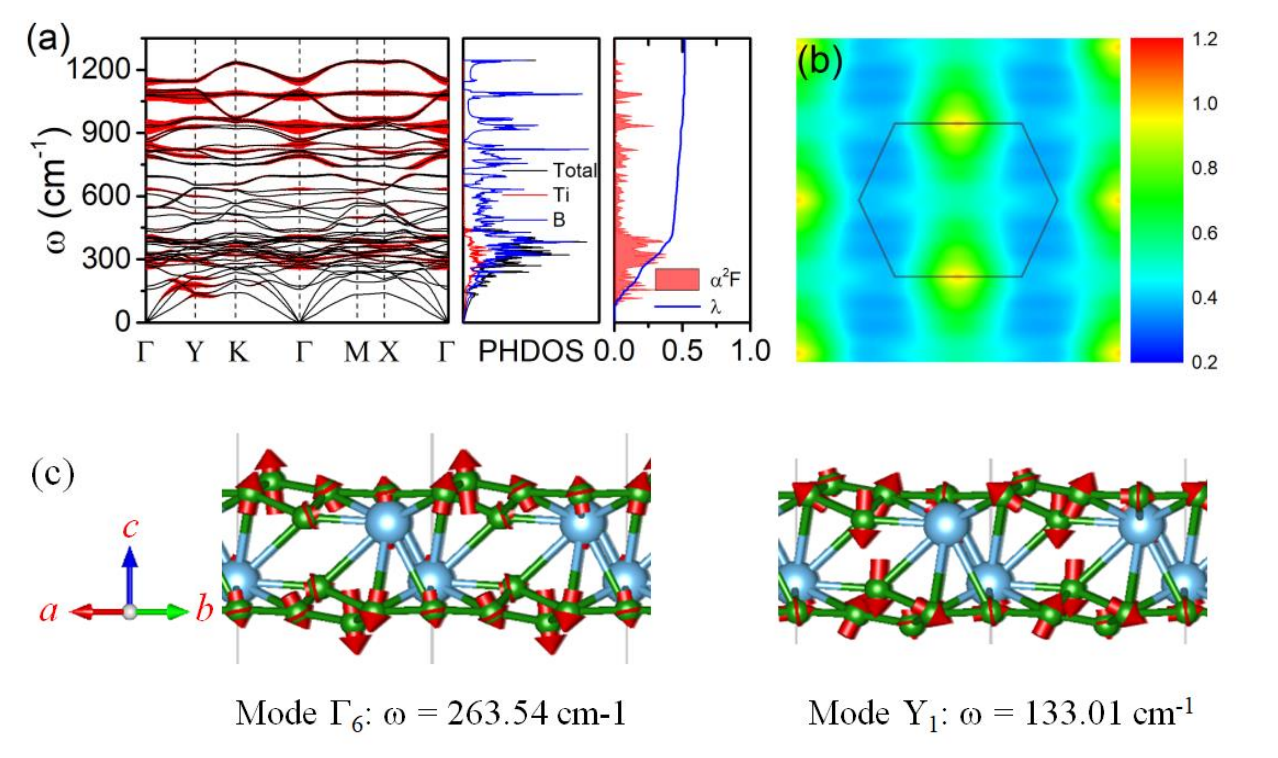
\includegraphics[width=0.96\textwidth]{figs/ch5_stack_tib7.png}
  \centering
  \caption{(a)(b)AB方式堆叠的\ce{TiB7}单层薄膜的声子色散以及声子线宽$\gamma_{qj}$、声子态密度、Eliashberg函数$\alpha^2 F(\omega)$和$\lambda(\omega)$和耦合常数强度在倒空间的分布。(c)振动模式$\Gamma_6$和$Y_1$的具体形式。}
  \label{fig:ch5_stack_tib7}
\end{figure}

图\ref{fig:ch5_stack_tib7}(b)中展示了电声耦合系数$\lambda_{\bm{q}}$在到空间中的变化情况,
我们可以看到,声子线宽在$Y$对称点附近为最大,这是与单层\ce{TiB7}所不同的,
且该处的电声耦合系数为最大值$\lambda_{\bm{q}}\approx 1$。
这使得原先单层中对电声有较大贡献的面内的旋转振动模式不再出现。与单层\ce{TiB7}相同,
双层\ce{TiB7}的电声耦合同样主要来源于原子质量较轻的硼原子。

\begin{table}[H]
  \centering
  \begin{tabular}{lllll}
    \hline\hline
    构型 & $N(\epsilon_F)$ & $\omega_\mathrm{log}$ & $\lambda$ & $T_c$(\si{\kelvin}) \\
    \hline
    \ce{TiB7}单层 & 1.78 & 290.47 & 0.65 & 8.3 \\
    \ce{TiB7}双层 & 1.32 & 409.90 & 0.51 & 5.5 \\
    \ce{TiB9}单层 & 2.25 & 325.97 & 0.40 & 1.2 \\
    \ce{TiB4}单层 & 1.21 & 484.87 & 0.18 & $\approx$ 0.0 \\
    \ce{Ti2B2}单层 & 7.96 & 326.75 & 0.27 & $\approx$ 0.0 \\
    \hline
  \end{tabular}
  \caption{各种二维钛硼结构的超导电性}\label{table:sc_all}
\end{table}

另外,我们也计算了其他钛硼二维材料的超导电性。
我们将本文所研究的和已经报导的钛硼结构的电声耦合和超导电性总结在表\ref{table:sc_all}中。
综上,我们共计算了单层\ce{TiB7}、单层\ce{TiB9},文献报导的单层\ce{TiB4}、单层\ce{Ti2B2},
以及我们根据单层\ce{TiB7}采用AB方式堆叠的双层\ce{TiB7}的超导电性。
其中,单层\ce{TiB7}的超导转变温度最大,达到了\SI{8.3}{\kelvin},\ce{TiB7}双层的超导转变
温度为\SI{5.5}{\kelvin},\ce{TiB9}单层的超导转变温度为\SI{1.2}{\kelvin}。
\ce{TiB4}和\ce{Ti2B2}单层虽然有较大的对数平均声子频率$\omega_{\mathrm{log}}$,
但电声耦合强度$\lambda$均太小,而无法体现超导电性。

\section{本章小结}

本章我们利用第一性原理方法,
计算并分析单层\ce{TiB7}最稳定构型的超导电性。
在不施加应力时,该构型的超导转变温度为\SI{8.3}{\kelvin},
高于文献报导的锂沉积石墨烯的超导转变温度\SI{8.1}{\kelvin}。
\ce{TiB7}的超导主要是由硼元素所贡献,
其电声耦合主要来自$\Gamma$点附件低频率范围的四种振动模式。
通过对该构型施加拉伸应变,我们发现超导转变温度随之减小。
可以将该单层\ce{TiB7}通过AB堆叠构成的双层\ce{TiB7}构型
该双层\ce{TiB7}构型也具有超导电性,
超导转变温度为\SI{5.5}{\kelvin}。

